\documentclass{standalone}

\usepackage{tikz}
\usetikzlibrary{backgrounds, positioning, shapes.symbols}
\usepackage{helvet}
\renewcommand*{\rmdefault}{\sfdefault}

\begin{document}
\begin{tikzpicture}
  [
    font=\footnotesize,
    faraday/.style={minimum size=3cm, draw, dashed},
    duplexer/.style={draw,fill=white},
  ]

  \node[faraday, label={[anchor=south east]above right:Faraday cage}] (faraday) {};

  \node[above left=0cm and 2.8cm of faraday, label=above:obelix] (obelix)
    {
\includegraphics[width=1.2cm]{server}};
  \node[right=0.3cm of obelix, label=above:B200-mini] (b210o)
    {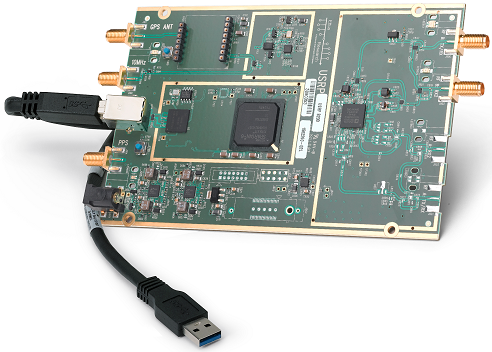
\includegraphics[width=1.2cm]{b200-mini}} edge (obelix);
  \node[below right=0.35cm of faraday.north west] (anto)
    {
\includegraphics[width=0.3cm]{antenna}};
  \draw (b210o) -| node [pos=0.2, duplexer] {B7} (anto);

  \node[below left=0cm and 2.8cm of faraday, label=above:nepes] (nepes)
    {
\includegraphics[width=1.2cm]{server}};
  \node[right=0.3cm of nepes, label=above:B200-mini] (b210n)
    {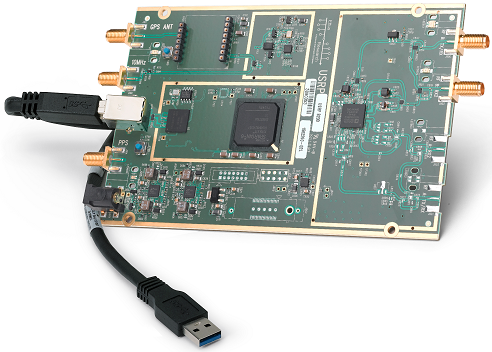
\includegraphics[width=1.2cm]{b200-mini}} edge (nepes);
  \draw (obelix) -- (b210o);
  \node[above right=0.35cm of faraday.south west] (antn)
    {
\includegraphics[width=0.3cm]{antenna}};
  \draw (b210n) -| node [pos=0.2, duplexer] {n78} (antn);

  \node[left=5cm of faraday, label=above:porcepix] (porcepix)
    {
\includegraphics[width=1.2cm]{server}};
  \draw (obelix) -- (porcepix);
  \draw (nepes) -- (porcepix);

  \node[right=1.5cm of faraday, label=above:RM500Q-GL] (quectel)
    {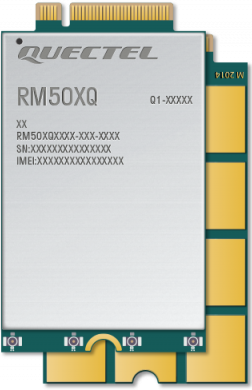
\includegraphics[height=1.2cm]{quectel}};
  \node[above left=-0.1cm and 0.2cm of faraday.east] (aq2)
    {
\includegraphics[width=0.3cm]{antenna}} edge (quectel);
  \node[above=-0.2cm of aq2] (aq1)
    {
\includegraphics[width=0.3cm]{antenna}} edge (quectel);
  \node[below=-0.2cm of aq2] (aq3)
    {
\includegraphics[width=0.3cm]{antenna}} edge (quectel);
  \node[below=-0.2cm of aq3]
    {
\includegraphics[width=0.3cm]{antenna}} edge (quectel);
  \node[right=1cm of quectel, label=above:idefix] (idefix)
    {
\includegraphics[width=1.2cm]{server}}
    edge (quectel);

\end{tikzpicture}
\end{document}
